%%%%%%%%%%%%%%%%%%%%%%%%%%%%%%%%%%%%%%%%%%%%%%%%%%%%%%%%%%%%%%%%%%%%
%% I, the copyright holder of this work, release this work into the
%% public domain. This applies worldwide. In some countries this may
%% not be legally possible; if so: I grant anyone the right to use
%% this work for any purpose, without any conditions, unless such
%% conditions are required by law.
%%%%%%%%%%%%%%%%%%%%%%%%%%%%%%%%%%%%%%%%%%%%%%%%%%%%%%%%%%%%%%%%%%%%

\documentclass[
  digital,     %% The `digital` option enables the default options for the
               %% digital version of a document. Replace with `printed`
               %% to enable the default options for the printed version
               %% of a document.
%%  color,       %% Uncomment these lines (by removing the %% at the
%%               %% beginning) to use color in the printed version of your
%%               %% document
  oneside,     %% The `oneside` option enables one-sided typesetting,
               %% which is preferred if you are only going to submit a
               %% digital version of your thesis. Replace with `twoside`
               %% for double-sided typesetting if you are planning to
               %% also print your thesis. For double-sided typesetting,
               %% use at least 120 g/m² paper to prevent show-through.
  nosansbold,  %% The `nosansbold` option prevents the use of the
               %% sans-serif type face for bold text. Replace with
               %% `sansbold` to use sans-serif type face for bold text.
  nocolorbold, %% The `nocolorbold` option disables the usage of the
               %% blue color for bold text, instead using black. Replace
               %% with `colorbold` to use blue for bold text.
  lof,         %% The `lof` option prints the List of Figures. Replace
               %% with `nolof` to hide the List of Figures.
  lot,         %% The `lot` option prints the List of Tables. Replace
               %% with `nolot` to hide the List of Tables.
]{fithesis4}
%% The following section sets up the locales used in the thesis.
\usepackage[resetfonts]{cmap} %% We need to load the T2A font encoding
\usepackage[T1,T2A]{fontenc}  %% to use the Cyrillic fonts with Russian texts.
\usepackage[
  main=english, %% By using `czech` or `slovak` as the main locale
                %% instead of `english`, you can typeset the thesis
                %% in either Czech or Slovak, respectively.
  english, german, russian, czech, slovak %% The additional keys allow
]{babel}        %% foreign texts to be typeset as follows:
%%
%%   \begin{otherlanguage}{german}  ... \end{otherlanguage}
%%   \begin{otherlanguage}{russian} ... \end{otherlanguage}
%%   \begin{otherlanguage}{czech}   ... \end{otherlanguage}
%%   \begin{otherlanguage}{slovak}  ... \end{otherlanguage}
%%
%% For non-Latin scripts, it may be necessary to load additional
%% fonts:
\usepackage{paratype}
\def\textrussian#1{{\usefont{T2A}{PTSerif-TLF}{m}{rm}#1}}
%%
%% The following section sets up the metadata of the thesis.
\thesissetup{
    date        = \the\year/\the\month/\the\day,
    university  = mu,
    faculty     = fi,
    type        = bc,
    department  = Department of Computer Systems and Communications,
    author      = Tomáš Zobač,
    gender      = m,
    advisor     = {RNDr. Rudolf Wittner},
    title       = {Implementation of provenance chains traversal},
    TeXtitle    = {Implementation of provenance chains traversal},
    keywords    = {Java, provenance, SOBHA, ÚVT},
    TeXkeywords = {Java, provenance, SOBHA, ÚVT},
    abstract    = {%
      Provenance is information documenting the history of an object. It can hold information, such as the origin of an object or previous actions performed on it. This information can be serialized into one of the many supported representations (e.g., PROV-N, XML) and subsequently interconnected, creating a provenance chain. This thesis aims to implement a tool for traversing provenance chains represented by PROV-N files, retrieving information about the precursors or successors of an entity represented in one of the files in the current chain, and optionally retrieving the type of actions performed on the object by the retrieved precursors/successors. The implementation will simulate the operational environment by providing a command-line user interface from where the user can call the mentioned actions on a set of pre-generated simulation files. Additionally to the traversing operations, it will also implement the generation of a provenance metadata to make the simulation of a traversal possible.
    },
    thanks      = {%
      TODO
    },
    bib         = citations.bib,
    %% Remove the following line to use the JVS 2018 faculty logo.
    facultyLogo = fithesis-fi,
}
\usepackage{makeidx}      %% The `makeidx` package contains
\makeindex                %% helper commands for index typesetting.
%% These additional packages are used within the document:
\usepackage{paralist} %% Compact list environments
\usepackage{amsmath}  %% Mathematics
\usepackage{amsthm}
\usepackage{amsfonts}
\usepackage{url}      %% Hyperlinks
\usepackage{markdown} %% Lightweight markup
\usepackage{listings} %% Source code highlighting
\usepackage{dirtree}
\usepackage{fancyvrb}
\lstset{
  basicstyle      = \ttfamily,
  identifierstyle = \color{black},
  keywordstyle    = \color{blue},
  keywordstyle    = {[2]\color{cyan}},
  keywordstyle    = {[3]\color{olive}},
  stringstyle     = \color{teal},
  commentstyle    = \itshape\color{magenta},
  breaklines      = true,
}
\usepackage{floatrow} %% Putting captions above tables
\floatsetup[table]{capposition=top}
\usepackage[babel]{csquotes} %% Context-sensitive quotation marks
\begin{document}
%% The \chapter* command can be used to produce unnumbered chapters:
\chapter*{Introduction}
%% Unlike \chapter, \chapter* does not update the headings and does not
%% enter the chapter to the table of contents. I we want correct
%% headings and a table of contents entry, we must add them manually:
\markright{\textsc{Introduction}}
\addcontentsline{toc}{chapter}{Introduction}
\shorthandoff{-}
Provenance, a term of significant importance in both historical and digital contexts, denotes the collective information regarding the origin and history of an object, idea, or data. Its relevance becomes particularly pronounced when objects or data are distributed across multiple organizations, each documenting only a part of its entire provenance. Such distributed provenance poses a unique challenge, especially in scientific research, where provenance can be used, for example, to verify the research's quality and reliability or to reproduce its results.

Current research \cite{research} focuses on the complexities of handling this distributed provenance where research objects are passed between various organizations, and no single organization possesses complete provenance of exchanged objects, leading to potential gaps in the research object's history and authenticity. The outcome of this research is a concept of a provenance chain, where the provenance documented by each organization is linked together to form a cohesive, traversable chain. This thesis aims to implement a command line tool to navigate these provenance chains and retrieve information about the precursors or successors of an object represented by an Entity from this chain. 

The first chapter describes the PROV-DM data model for provenance information representation and its expression through the PROV-N notation, developed by the World Wide Web Consortium (W3C). Furthermore, it describes the provenance chain and additional concepts tied to it. The second chapter delves into the design of the implemented tool, follows with an insight into how the real-world environment is simulated, and ends with an explanation of the provenance chain traversal. The third chapter describes the implementation's technicalities, structure, and execution, with the last chapter serving as a manual on how to set up and run the implemented tool.
\shorthandon{-}

\chapter{Provenance}
This chapter begins by delving into the PROV-DM data model developed by the World Wide Web Consortium (W3C), offering insights into how provenance information is represented, organized, and utilized in a digital environment. The chapter introduces PROV-N, a notation for expressing provenance data, illustrating its structure and application with practical examples. After this, it introduces the concept of a provenance chain and provides an example of real-world application in medical research. The chapter concludes by introducing additional concepts of meta-provenance and resolution of persistent identification, all central to this thesis.

\section{PROV-DM} \label{provdm}
\shorthandoff{-}
The W3C PROV-DM (Provenance Data Model) standard \cite{provdm} was created to enable the inter-operable interchange of provenance information. The PROV-DM represents provenance as a directed graph. 

\begin{figure}[htbp]
  \begin{center}
    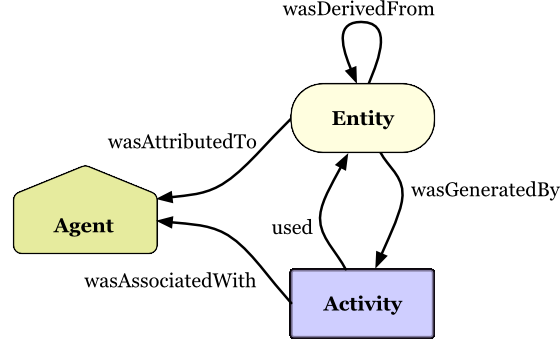
\includegraphics[width=10cm]{fithesis/images/provdm-basics.png}
  \end{center}
  \caption{High level overview of the structure of PROV records \cite{provdm-basics}}
  \label{fig:provdm-basics}
\end{figure}

Nodes in a provenance graph represent three types of objects that can be expressed in provenance: Entities, Activities, and Agents. Entities represent snapshots of physical, digital, or other objects central to or associated with the provenance, taken at a concrete point in time. Activities represent actions and processes conducted on or with these entities. Agents are the nodes that perform activities, effectively creating or influencing entities and activities. The edges in a provenance graph represent the relations between these nodes, with examples being 'wasDerivedFrom,' 'wasGeneratedBy,' and 'used.' Both nodes and edges can be referred to as provenance structures. Each provenance structure has properties the model defines, attributes the user defines, and a unique identifier, which identifies it in the current provenance graph. The identifier is a QualifiedName, which consists of the name of the object it refers to, a namespace that categorizes or contains it, and an optional prefix to represent the namespace more concisely. The PROV-DM supports extensions of its base model, with the users being able to define new types of nodes and edges and add custom attributes; this enhances the flexibility of the PROV-DM.

Moreover, the PROV-DM standard includes a concept known as Bundles, which are used to group sets of provenance structures. Like other provenance structures, a Bundle also has a QualifiedName identifier, which allows it to be represented in a provenance as an Entity, effectively allowing the creation of a provenance of a provenance.
\shorthandon{-}

\subsection{PROV-N}
\shorthandoff{-}
PROV-N \cite{provn} is a component of the W3C PROV suite, designed to represent PROV-DM in a human-readable textual format, using files with .provn extension. Each PROV-N file contains a single Document organized into three main sections: namespace declarations, statements, and bundles. A PROV-N document, with declared namespaces and a bundle encapsulating its statements, could look like this snippet: 

\begin{center}
\begin{lstlisting}[numbers=left,
    stepnumber=1,
    tabsize=4,
    breaklines=true,
    breakatwhitespace=false,
    xleftmargin=3.5em
    ]
document
  prefix prefix1 <prefix1_URI>

  bundle prefix1:sampleBundle.provn
    prefix prefix1 <prefix1_URI>
    prefix dct <dct_URI>

    entity(prefix1:entity1,[
        prov:type='image',
        dct:format='jpeg',
    ])
  endBundle
endDocument
\end{lstlisting}
\end{center}

Namespace declarations (lines 2, 5, and 6 of the snippet) are a technical means to define qualified names in PROV-N Documents. They shorten the QualifiedName identifiers by specifying a shorthand prefix to a longer namespace URI at the beginning of each Document and Bundle. For instance, a QualifiedName of the Entity from the snippet (line 8) will look as follows:

\begin{verbatim}

    prefix1:{{prefix1_URI}}entity1
    
\end{verbatim}

Statements represent provenance structures. For example, the Entity from the snippet (line 8 of the snippet) is described as "entity(QualifiedName identifier)" with property (line 9 of the snippet) specifying that the documented object is an image and attribute (line 10 of the snippet) detailing its characteristics.

Bundles (line 4 of the snippet) are optional functionality for grouping provenance structures. Provenance structures can be defined outside or inside of a Bundle, but Bundles themselves cannot be folded into each other. Because the QualifiedName of the Bundle from the snippet contains the prefix "prefix1", it must also be declared outside of the Bundle (line 2 of the snippet).
\shorthandon{-}

\section{Provenance chain} \label{s-provchain}
\shorthandoff{-}
The provenance chain is defined in the Common Provenance Model \cite{cpm}, an extension of the PROV-DM for distributed environments. It is defined as a sequence of interconnected Bundles, each encapsulating a graph consisting of two parts. The first part is a provenance backbone, a part of the Bundle's graph that serves as a guide for traversing provenance chains; it contains information about the graph in the given Bundle and establishes connections within and between Bundles. Each Bundle in the provenance chain refers to an activity that takes inputs and produces outputs. Backbone has a pre-defined structure for mapping these inputs to outputs. Therefore, the content of the backbone is not dependent on what specific type of activity is documented.

The second part is a domain-specific part of the graph. It is a more detailed description of the activity documented in the Bundle; it gives more detailed information compared to what is stored on the backbone. Provenance backbone and domain-specific information are linked in a contiguous graph in a defined way, which is out of the scope of this thesis. This thesis will work only with a part of the provenance backbone relevant to it.

The provenance backbone, as shown in Figure \ref{fig:bundleconnection}, comprises three types of Entities: backwardConnector, currentConnector, and forwardConnector. These Entities are related to each other through the WasDerivedFrom derivation.  

\begin{figure}[htbp]
  \begin{center}
    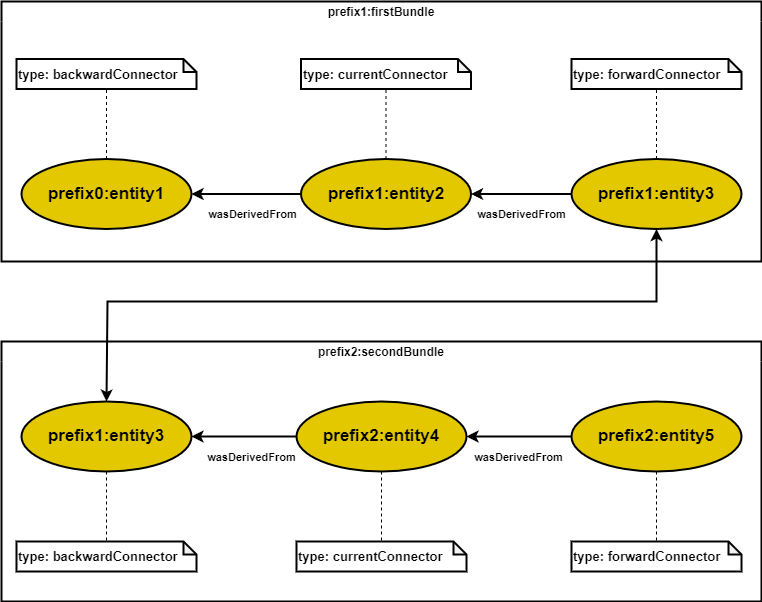
\includegraphics[width=12.5cm]{fithesis/images/backbone.png}
  \end{center}
  \caption{Example of a provenance backbone}
  \label{fig:bundleconnection}
\end{figure}

The backwardConnector represents the documented object at the time it was sent from the sender to the receiver and references the previous Bundle in the chain, where it links to a forwardConnector with the same identifier.

The currentConnector, derived from the backwardConnector, represents the documented object at the time the receiver Bundle received it and references the current Bundle.

The forwardConnector, derived from the currentConnector, represents the documented object at the time it was sent from the current Bundle and references the succeeding Bundle in the chain, where it links to a backwardConnector with the same identifier. If graphs of two succeeding Bundles were to merge, the point of connection of these graphs would be their linked forwardConnector and backwardConnector, both representing the documented object at the same time instant.

The end of the provenance chain can be recognized by connectors missing from a Bundle's backbone. A Bundle missing the backwardConnector and currentConnector represents a starting point in the provenance chain, while a Bundle missing the forwardConnector represents the endpoint. \cite{provchain}

While the example from Figure \ref{fig:bundleconnection} simplifies the structure, in practice, a single bundle can contain multiple connectors of the same type. This multiplicity allows connections to more than one Bundle on either side of the provenance backbone, thereby accommodating complex provenance scenarios.

\shorthandon{-}

\section{Real-world distribution}
The provenance chain is meant to be used in a multi-organizational distributed environment, meaning the bundles of a provenance chain are distributed across multiple companies and that one or more Bundles from the chain represent a company's processing of the provenance's object, effectively documenting its complete lifecycle.

\label{t-aiexample} This thesis works with an example of a provenance chain consisting of six Bundles, documenting a process of training an AI model to detect tumors on images of prostate tissue. Each Bundle from this provenance chain documents part of the process. The first Bundle documents the collection of a sample. The second Bundle documents the diagnosis and data generation. After this, the chain branches out as the third Bundle documents the storage of the sample in a biobank, while the chain continues into the fourth Bundle, documenting the preprocessing of the generated data for AI model training. The fifth Bundle documents the process of the AI model training, and the last Bundle documents the testing of the trained AI model. See the Running example section in \cite{research} for more details.

\section{Additional concepts}
Additional concepts were developed in order to address issues that tie to the usage of the provenance chain in a distributed environment. One such issue is how to account for versioning of Bundles in the chain. To address it, the meta-provenance is used. Meta-provenance is a Bundle that keeps provenance, like the current version and its hashes, about the Bundles, ensuring that each one links to the correct version of the succeeding Bundles. \cite{metaprov}

Another concept is the usage of persistent identification (PID). 
The PID \cite{pid} is:

\begin{enumerate}
    \item Globally unique, meaning that it is distinct and distinguishable from all other identifiers across the globe, with no two entities having the same PID.
    \item Persistent, meaning that it ensures that the link to the data or resource remains constant over time, regardless of any changes.
    \item Resolvable, meaning that the PID can be used to locate and access the resource it identifies.
\end{enumerate}

PID management is usually performed by an external service, where users can register new PIDs by defining what the PID will resolve into. In the case of provenance chains, the PID resolves into a quartet of values:

\begin{enumerate}
    \item Entity ID
    \item Connector type of the Entity
    \item ID of a Bundle referenced by the Entity
    \item ID of meta-provenance containing the referenced Bundle
\end{enumerate}

The goal of the PID in provenance chains is to support the validity of the connector identifiers in the long term, i.e., that the links to the other bundles and related information are not deprecated. 


\chapter{Design}
\shorthandoff{-}
This chapter delves into the architecture and logic of the command line tool and its underlying library, both developed as an implementation part of this thesis. The chapter has three main objectives. Firstly, it aims to provide a clear and concise overview of the implementation structure and its components, including their respective roles in its lifecycle. Secondly, it discusses the simulated environment of a real-world distribution and how it works. Finally, it describes the primary logic used to traverse a provenance chain. 
\shorthandon{-}

\section{Overview}
Thanks to its command line interface, the implementation allows users to perform different operations by entering their associated commands. The main operation is to provide the user with the ability to retrieve precursors or successors of an Entity in a provenance chain. \ref{t-aiexample} The secondary operation is to retrieve the precursors or successors together with the main activity of their Bundles. The additional operations are to print this implementation's navigational table and to resolve data for an Entity from the mentioned table.

A bonus feature of the implemented command line interface is that it serves as a code reference for anyone who wants to use one or more library components for their project. By looking at the code of the interface, any interested party can gain insight into how and where to initialize and use the library's components for their intended results.

Furthermore, the implementation contains a secondary library used to generate meta-provenance to keep the provenance of Bundles in the chain with their hashes. This secondary library is used only for the simulation, to be described in \ref{s-simulation}.

\section{Structure}
\shorthandoff{-}
The implementation is designed as a modular, multi-component library. Central to this structure is a layered architecture, segregating the library operations into distinct layers - data retrieval, processing, and presentation. 

The data retrieval layer is responsible for loading and deserializing the PROV-N files, depending on the type of storage. 

The processing layer handles the traversal of the provenance chain as well as the traversal of the provenance backbone inside each PROV-N document. It is also responsible for verifying the integrity of documents and retrieving data from the navigational table and meta-provenance.

Finally, the presentation layer provides the interface for user interaction, enabling the user to enter commands and display results on the command line.
\shorthandon{-}

\subsection{Components}
\shorthandoff{-}
The library's components are separated into four main parts.
\begin{enumerate}
    \item \textbf{Main UI:}
        The Main UI component is tasked with the initialization of resources for the library and providing a user interface on the command line, where the user can input commands and view the results of the entered queries. The user interface also provides quality-of-life functions, such as command auto-completion, command history, or in-command query history.
    \item \textbf{Configuration:}
        The Configuration component retrieves data from a configuration JSON file and passes it to the library.
    \item \textbf{Tools:}
        The Tools component serves as a toolset for the library, with the first set of tools used to retrieve and deserialize PROV-N documents depending on their storage type. 
        The second set of tools is used to resolve persistent identifiers stored in the relevant navigation table.
        The third is used for retrieving hash values from the corresponding meta-provenance, and the last is used for hash creation and integrity verification.
    \item \textbf{Main logic:}
        The Main logic component handles the data processing. It traverses the provenance chain and retrieves the user-specified data. It also assures the correctness of the traversed chain by evaluating the integrity of the document using its hash values stored in the corresponding meta-provenance and comparing it to new hash values created using the last set of tools.
\end{enumerate}
\shorthandon{-}

\section{Simulation} \label{s-simulation}
\shorthandoff{-}
For the implementation to provide a more focused simulation of a real-world environment, some limitations had to be established specifically for this thesis. The simulation of a distributed environment is performed on a set of prepared files. The thesis supervisor provided this set comprising 6 PROV-N files, each containing a single Bundle pre-filled with domain-specific data and a provenance backbone defined in \ref{s-provchain} to form a provenance chain. This provenance chain represents a process from digital pathology, where a biological sample is retrieved from a patient, to be then processed for the generation of image data, which is then used as input for the training of artificial intelligence. The described process consists of 6 steps, with each step being documented in one of the Bundles from the chain. The simulation itself is achieved by a recursive call of the Main logic on this provenance chain. In contrast, in a real-world environment, this Main logic would exist, for example, in a public API of a service deployed in multiple instances. 

Because when the work on this thesis began, the concept of provenance chains was a state-of-the-art solution for the representation of distributed provenance, the way PID resolution and meta-provenance were going to work still needed to be decided. Both had to be implemented in this thesis to overcome this issue and simulate their existence in a real-world environment. For meta-provenance, a second library was implemented. This library generates a single meta-provenance containing all Bundles from the chain, along with their hashes, which it also generates using the Tools for hash creation. To simulate PID resolution, an in-memory implementation of a navigational table is used. This table consists of all Bundles in the chain, and access to it is implemented through the PID resolution Interface. The inclusion of this Interface allows the implemented library to be extended to other types of PID resolution and navigational tables.
\shorthandon{-}

\section{Provenance chain traversal}
\shorthandoff{-}
This section discusses the traversal of the provenance chain using the provenance backbone and retrieval of precursors or successors of an Entity. The inputs for this traversal are a QualifiedName identifier of an Entity and a QualifiedName identifier of a Bundle containing the Entity. In this example, the traversal moves in a forward direction, retrieving the successors of the Entity. The successors are represented by backwardConnectors. The inputs are prefix1:entity1, which is a forwardConnector from prefix1:bundle1, and the provenance chain has a structure, as shown in Figure \ref{fig:algorithm-Chain}

\begin{figure}[htbp]
  \begin{center}
    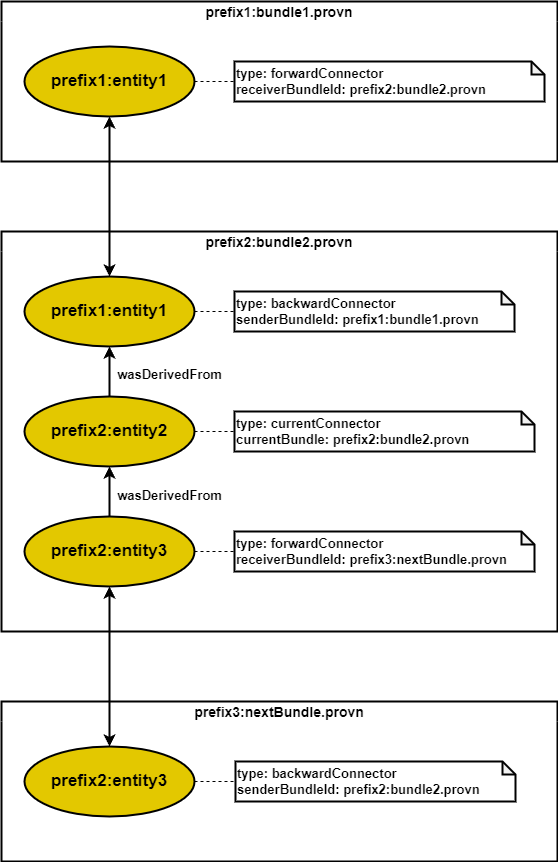
\includegraphics[width=11.5cm]{fithesis/images/algorithm-Chain.png}
  \end{center}
  \caption{Example of the provenance chain's structure}
  \label{fig:algorithm-Chain}
\end{figure}
\shorthandon{-}

Considering the traversal is already at the end of the bundle1's backbone, the next step is to move to the Entity linked to the entity1, which is an Entity with the same identifier in the bundle2. An example shown in Figure \ref{fig:algorithm-BundleLink}

\begin{figure}[htbp]
  \begin{center}
    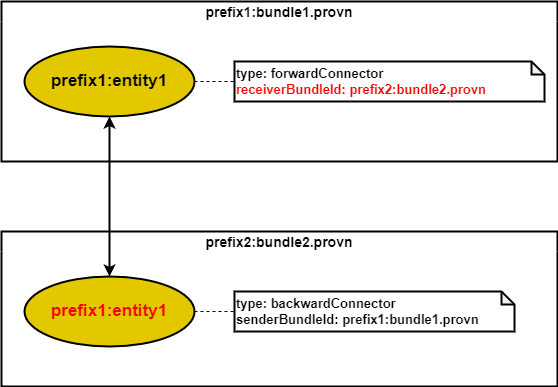
\includegraphics[width=12cm]{fithesis/images/algorithm-BundleLink.png}
  \end{center}
  \caption{Moving between two linked Bundles}
  \label{fig:algorithm-BundleLink}
\end{figure}

Because the traversal is currently on a backwardConnector, the current Entity and Bundle identifiers are returned, as shown in Figure \ref{fig:algorithm-Result}, and the traversal continues.

\begin{figure}[htbp]
  \begin{center}
    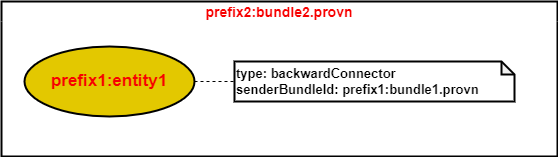
\includegraphics[width=12cm]{fithesis/images/algorithm-Result.png}
  \end{center}
  \caption{QualifiedNames of the current Entity and Bundle}
  \label{fig:algorithm-Result}
\end{figure}

The next step is for the traversal to move using the wasDerivedFrom edge onto the following Entity, which is a currentConnector, and then move again using the wasDerivedFrom edge to arrive on a forwardConnector. The traversal moves into the next Bundle, and the whole process repeats, retrieving the next successor. An example shown in Figure \ref{fig:algorithm-Continue}

\begin{figure}[htbp]
  \begin{center}
    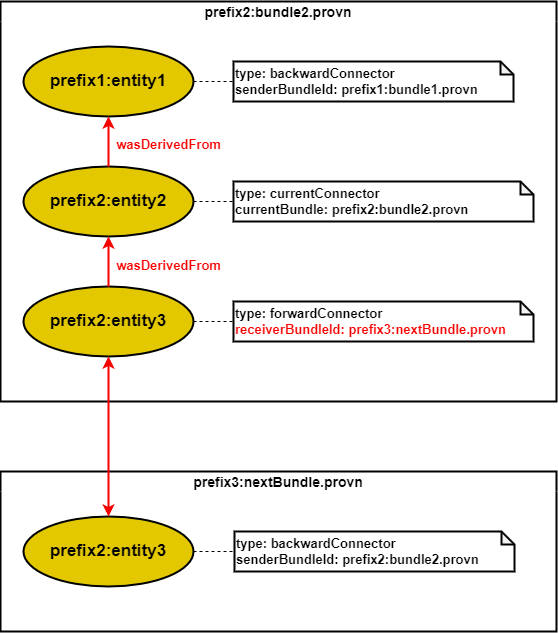
\includegraphics[width=12cm]{fithesis/images/algorithm-Continue.png}
  \end{center}
  \caption{Traversal of the Bundle's backbone}
  \label{fig:algorithm-Continue}
\end{figure}

The traversal ends when no more Entities are derived using the wasDerivedFrom edge, or there are no succeeding bundles.


\chapter{Implementation}
\shorthandoff{-}
This chapter aims to establish a connection between the theoretical framework discussed in the Design chapter and the practical implementation of the project. Firstly, it offers an in-depth look at the code structure. After that, it provides a listing of used libraries and a description of their usage in the implementation. It follows with a description of the implementation's runtime and finishes with a section about problems that arose during the implementation.

\section{Used technologies}
The following part delves into the libraries and tools used in the implementation and the reasoning behind the usage of each.
\subsection{ProvToolBox}
The ProvToolBox library \cite{provtoolbox} is a cornerstone for managing provenance data within the implementation. It provides multiple sublibraries, each focusing on some aspect of provenance management in the code. Two of these sublibraries, the prov-model, and prov-interop-light, are used in this implementation. The prov-model is used across the whole implementation to create and manipulate provenance documents. Complementary to the prov-model, the prov-interop-light enhances the system's interoperability. This library facilitates the conversion of provenance data into various formats, ensuring that the application can communicate effectively with other provenance-aware systems and tools.
\subsection{Jackson Databind}
Jackson Databind \cite{jackson} is a library for handling JSON data formats. In ConfigLoader.java and Configuartion.java, 'jackson-databind' parses the configuration file and creates Java objects from JSON. This functionality is crucial in managing configurations within the library.
\subsection{GitLab4J API}
Integrated primarily in GitLabFileLoader.java, the GitLab4J API \cite{gitapi} is a library to facilitate interaction with GitLab's APIs. It automates file retrieval, allowing the library to support git-based provenance storage.
\subsection{JLine Bundle}
JLine Bundle \cite{jline} is a library used to enhance the user interface of the implementation, as seen in MainRuntime.java. It provides capabilities such as command-line completion and history, significantly improving the user experience by making the interface more intuitive and responsive.
\subsection{Jansi}
Utilized in MainRuntime.java, Jansi \cite{jansi} is a library used to improve formatting options of the console output. It renders text in different colors and styles, making the console output about the integrity of Bundles more readable and user-friendly.
\subsection{Apache Maven Shade Plugin}
The Maven Shade Plugin \cite{maven-shade} plays a significant role in the library's build process. This plugin creates an uber-jar, a standalone executable jar file containing all the necessary dependencies. This approach simplifies deployment and distribution, ensuring the library is self-contained and can be run in diverse environments without additional dependency management.
\section*{}
Each library has been chosen and integrated into the implementation to address specific functional requirements and enhance the application's usability, efficiency, and interoperability. The strategic use of these libraries aligns with the broader goal of creating a user-focused, adaptable, and future-proof application.

\section{Project structure}
\subsection{Configuration}
\dirtree{%
.1 provenancechain.
.2 config.
.3 ConfigLoader.java.
.3 Configuration.java.
.2 ....
}
\vskip 0.35cm

The configuration package comprises two classes for loading configuration data from a JSON file using the Jackson Databind library. The ConfigLoader class contains the main logic for JSON file deserialization. On the other hand, the Configuration class specifies the data type or object that the deserialized data will be cast into, depending on their name.

\subsection{Tools}
\dirtree{%
.1 provenancechain.
.2 ....
.2 tools.
.3 loading.
.4 ....
.4 IFileLoader.java.
.4 LoaderResolver.java.
.4 SupportedExtensions.java.
.3 metadata.
.4 IPidResolver.java.
.3 retrieving.
.4 IMetaHashRetriever.java.
.3 security.
.4 HashDocument.java.
.4 IntegrityVerifier.java.
}
\vskip 0.35cm

The tools package consists of four sub-packages, each with a set of specific tools. 

The loading sub-package consists of tools used for file retrieval. The IFileLoader interface is used to implement file retrieval depending on the type of storage, with current implementations being for GitLab and the local file system. Supplementary to the interface, the LoaderResolver class is used to choose the correct interface implementation, and the SupportedExtensions enum is used to avoid unsupported file types. 

The metadata sub-package consists of an IPidResolver interface used to implement resolving and access to the navigational table for different types of PIDs. 

The retrieving sub-package consists of an IMetaHashRetriever interface used to implement retrieval of hash values depending on the meta-provenance that contains it. 

Lastly, the security sub-package consists of tools used for operations with hashes. The HashDocument contains methods to create hashes for Documents, with SHA-256 and MD5 currently being the only techniques supported. The IntegrityVerifier class contains a static method to compare existing hashes from meta-provenance with newly created ones.

\subsection{Simulation}
\dirtree{%
.1 provenancechain.
.2 ....
.2 simulation.
.3 ....
.3 Initializer.java.
.3 SimulationFiles.java.
.2 ....
}
\vskip 0.35cm

The simulation package is used to hold implementations of interfaces from the tools package and other classes explicitly used for the simulation in this thesis. The SimulationFiles class is similar in structure to the IFileLoader implementations in the loading sub-package. However, it is used to load and prepare copies of the provided files saved in the project's resources to be used for simulation purposes. The Initializer class represents the building process of the simulation. It uses the SimulationFiles class to retrieve the required files and uses them to generate a meta-provenance and to create a navigational table. It also provides a static method to access this navigational table.

\newpage
\subsection{Main logic}
\dirtree{%
.1 provenancechain.
.2 ....
.2 logic.
.3 data.
.4 ProvenanceNode.java.
.3 Crawler.java.
.2 ....
.2 MainRuntime.java.
}
\vskip 0.35cm

The logic package and the MainRuntime class serve as the main logic of the implementation. The MainRuntime has a static constructor to initialize required resources for the implementation to work and provides a user-friendly command line interface for the user to enter commands. The supported commands are:

\begin{enumerate}
    \item "exit" to exit the program
    \item "precursors"/"successors" to print the precursors or successors of an Entity
    \item "precursors-activity"/"successors-activity" to print the precursors or successors of an Entity with the inclusion of the main Activity for each Bundle
    \item "resolve" to retrieve data from the navigational table for a specified Entity.
    \item "list" to print out the whole navigational table
    \item "help" to list all supported commands.
\end{enumerate}

The Crawler class contains the methods for traversing the provenance chain and retrieving the precursors or successors. The ProvenanceNode record is a direction-neutral representation of a node in the provenance graph and, therefore, can be used to store and represent the retrieved precursors or successors.

\section{Execution walkthrough}
This section is intended to provide a concise walkthrough of the implementation's execution. The purpose is to offer insight into how different classes and components interact to produce the desired results for the user. By following this walkthrough, readers will understand the underlying mechanisms of the operations performed during the execution. 

The execution begins by calling the method main in the class Main. The static initialization from the MainRuntime class is performed, followed by the calling of its run method.

\subsection{Initialization}
The static initialization performed by the MainRuntime class consists of three parts. The first part is the retrieval of data from the configuration JSON file. The second part is the initialization of the simulated environment. This part loads the provided provenance files, which are saved in the project resources. These files are then used to generate a meta-provenance using the sublibrary described in \ref{s-simulation}. In addition to generating the meta-provenance, this part also generates a simulated navigational table using the same files. The last part is the initialization of the remaining resources for the implementation to work.

\subsection{Runtime}
After calling the run method from the MainRuntime class, a command line interface is provided for the user to enter commands. For this walkthrough, the request is to retrieve the precursors of an Entity by using the 'precursors' command. The mentioned precursors are represented by the QualifiedName identifiers of forwardConnector Entities of the preceding Bundles. Refer to \ref{fig:runtime} for a better picture of the runtime.

\begin{figure}[htbp]
  \begin{center}
    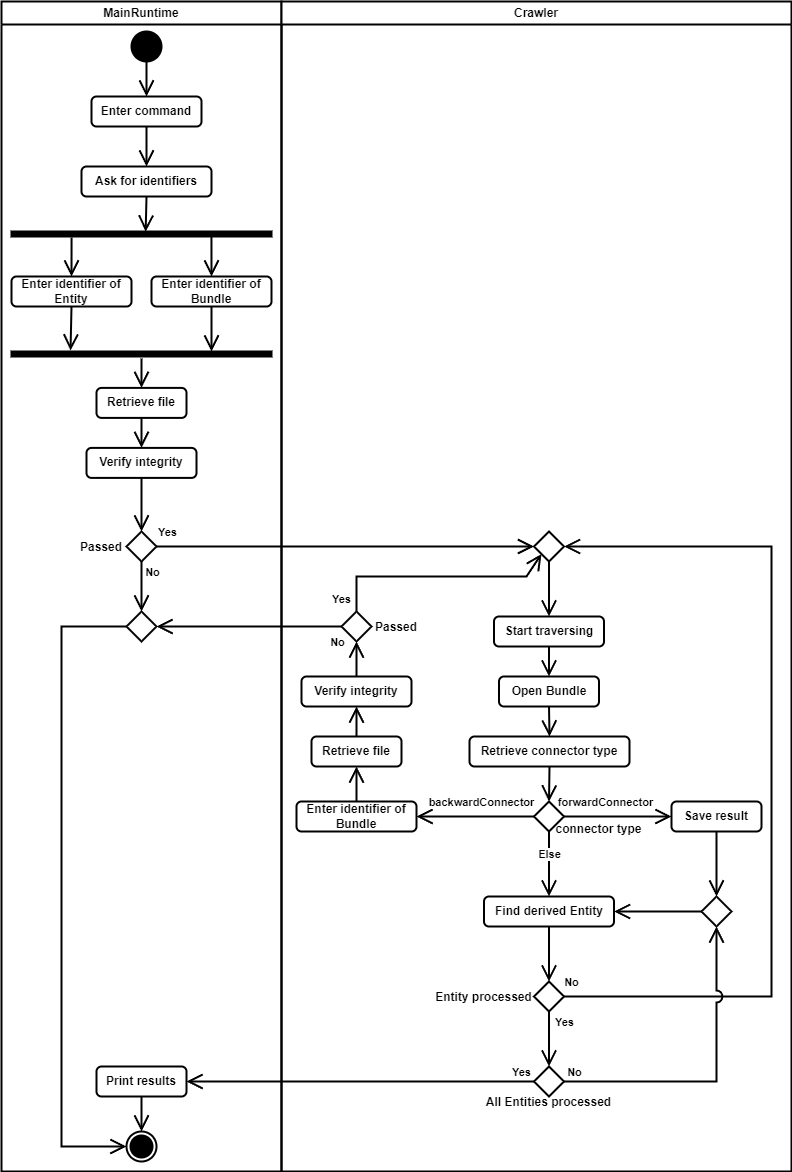
\includegraphics[width=12cm]{fithesis/images/precursorsactivity.png}
  \end{center}
  \caption{High level Activity diagram of the 'precursors' command}
  \label{fig:runtime}
\end{figure}
 
Afterward, the user is prompted to enter a connector's ID and URI and the ID and URI of a Bundle whose backbone contains the entered connector. Next, the correct implementation of the IFileLoader interface is chosen depending on what type of storage the Bundle's URI is pointing to, and the PROV-N file, with a name matching the Bundle's ID, is returned deserialized into a Document object. After that, the integrity of the Document is verified by calling the static checkSum method of the IntegrityVerifier class. This method compares this Document's newly created hash with its hash in the meta-provenance. With a successful integrity verification, the runtime enters the Crawler's method getPrecursors.

Upon entering, the proper navigational table resolver is chosen using the getPidResolver method. As part of the simulation in this thesis, the getPidResolver method is set to always return the simulated resolver. Next, the Bundle inside of the Document is retrieved and the type of the current connector is found. 

If the type is a forwardConnector, the connector's identifier and its Bundle's identifier are added to the list of precursors. The connector's identifier is also added to the list of processed nodes, and the method continues. 

If the type is a backwardConnector, it means the method reached the end of the current Bundle's backbone, and the same process as in the MainRuntime section repeats. The method uses the connector's entry in the navigational table to retrieve the identifier of the Bundle to which the connector is pointing. The following Document is retrieved using this information, and its integrity is again verified. The connector's identifier is added to the list of processed nodes, and the getPrecursors method is called with the same connector's identifier and the newly loaded Document. 

If the type is neither, the method will search through the WasDerivedFrom statements in the current Bundle to find which connector is following in the traversal. It will then add this connector's identifier to the list of processed nodes and call the getPrecursors method with the current Document and the newly found connector's identifier. 

After the runtime processes all Bundles in the chain and there are no more unprocessed connectors to enter, the traversal ends. The retrieved precursors are then printed on the command line, along with confirmation of the verified integrity of each Bundle. For an example, see Figure \ref{fig:precursor-run}. It should be mentioned that the implementation expects the chain to be correct, as the thesis supervisor stated that it should not focus on verification of whether the chain is cycled.

\begin{figure}[htbp]
  \begin{center}
    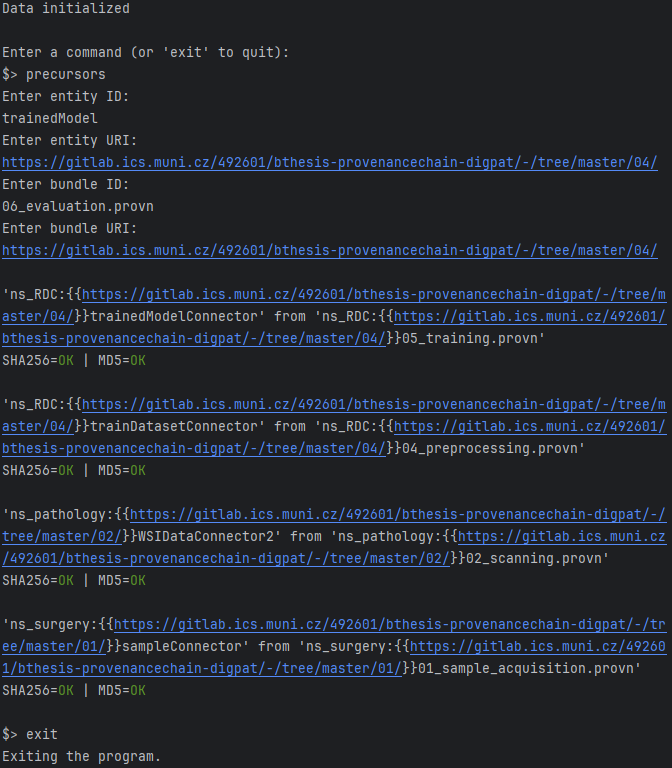
\includegraphics[width=12.5cm]{fithesis/images/precursor-run-slim.png}
  \end{center}
  \caption{Example of execution with the 'precursors' command}
  \label{fig:precursor-run}
\end{figure}

\section{Problems during implementation}
Four problems were encountered during the implementation due to using the ProvToolBox Java library. The first three problems arose from the simulation files, provided by the thesis supervisor, being generated using a Python library, which produced files with some notation differences. The first is that the Python library supports attributes with multiple values using parentheses, while the Java library needs each attribute to have only one value.

\begin{verbatim}

    Python: 
        dct:hasPart=('prefix:local','prefix:local')
    Java:
        dct:hasPart='prefix:local', 
        dct:hasPart='prefix:local' 
        
\end{verbatim}

The second problem came from the Python library supporting the creation of Entities with space in names, which is seen as a syntax error by the Java library.

\begin{verbatim}

    Python:
        entity(prefix:local 1, [prov:type=...
    Java:
        entity(prefix:local_1, [prov:type=... 
        
\end{verbatim}

The third problem was caused because the Python library generates attributes with values encompassed by double quotes. The Java library differentiates between single and double quotes. The single quotes are resolved as the QualifiedName specified inside of them.

\begin{verbatim}

    cpm:receiverBundleId='prefix:local.provn'
    
    Resolved:
        'prefix:{{uri}}local.provn'
        
\end{verbatim}

While the double quotes are regarded as a LangString

\begin{verbatim}

    cpm:receiverServiceUri="#URI#"
    
    Resolved:
        LangString@xxx[value=#URI#,lang=<null>]
        
\end{verbatim}

These findings about the libraries' differences were then reported to the thesis supervisor and were corrected in the provided files to use the Java-compatible notation.

The last problem came from the fact that the ProvToolBox library, at the time of thesis implementation, was left on version 0.9.3, with the last update being over three years ago, which caused some of the library's features not to work correctly or at all. One such feature was a method getEntity used to return an Entity with specified QualifiedName from a Bundle. The library's GitHub page had an open issue from 2019 about a similar method used to return an Agent instead of an Entity. To possibly remind the authors about the issue, a reply was posted as the specifications in the issue also applied to the getEntity method. The absence of this method in the implementation was compensated by looping over the Entities inside of a Bundle and finding the Entity with the same identifier. As of the late summer of 2023, the development seems to have returned, with new updates being released, and the mentioned issue being resolved and closed.
\shorthandon{-}


\chapter{Manual}
\shorthandoff{-}
\section{Set-up}
To utilize the implemented tool, it is necessary to have Maven and Java properly configured. To simplify the process for users, the implementation is currently spread across multiple Git repositories, including two on FI \cite{provchain-fi} and ICS \cite{provchain-ics} GitLab sites and one on the author's personal GitHub page \cite{provchain-github}. To obtain the tool, clone the repository or use the download button to retrieve the entire repository bundled in a zip or another archive file.

\subsection{Simulating the environment}
The initiation of simulation files is the first step in simulating the environment. It requires the retrieval of specific files necessary for the simulated environment to function effectively. To achieve this, a submodule in the repository must be initialized. Start by opening the cloned repository in a command line and navigating to the submodule's folder using the following command.

\begin{verbatim}
$ cd. \src\main\resources\bthesis-provenancechain-digpat  
\end{verbatim}

Once the submodule is reached, the command 

\begin{verbatim}
$ git submodule foreach git fetch –tags
\end{verbatim}

should be executed. After it finishes, there should be no output. Finally, the command

\begin{verbatim}
$ git submodule update --init --recursive  
\end{verbatim}

should be run to conclude the process. This will ensure that the bthesis-provenancechain-digpat submodule contains the required .provn files.

\section{Building}
The jar file is packaged using the Maven Shade plugin, which is the preferred method. To create the jar file, navigate to the cloned repository using the console and run the \textbf{\texttt{'mvn clean package'}} command. After creating the jar file, it can be launched by executing the command \textbf{\texttt{'java -jar }\path{.\target\BThesis-ProvenanceChain-VERSION-shaded.jar'}}. In the event that the intended environment does not have a JRE, the \textbf{\texttt{'jpackage'}} command line tool provided by Java can be used to create a platform-specific installer.

\section{Omitting the simulated environment}
To facilitate traversal simulation, the implementation employs several classes and files that provide the necessary objects for the algorithm to function. These classes have been transferred to packages labeled 'bthesis.provenancechain.simulation' and 'bthesis.metageneration' to enhance clarity. At the same time, the required files reside in the previously mentioned submodule 'src.main.resources.bthesis-provenancechain-digpat'. However, these components can be omitted if the required classes are adequately substituted.
\shorthandon{-}


\chapter*{Conclusion}
\markright{\textsc{Conclusion}}
\addcontentsline{toc}{chapter}{Conclusion}
\shorthandoff{-}
This thesis aims to develop and implement a command line tool for traversing provenance chains, beginning with an in-depth exploration of the provenance chains, PROV-DM data model, and PROV-N notation.

The design and implementation phase of the project emphasized creating a modular, multi-component library with a user-friendly command-line interface. This approach ensured adaptability and ease of use. The usage of various libraries, such as ProvToolBox, GitLab4J API, and others, exemplified the seamless integration of different technologies to achieve the desired functionality. The execution walkthrough highlighted the dynamic interaction of various system components, demonstrating the implementation's practicality and robustness. The problems encountered during implementation, mainly related to the ProvToolBox Java library, provided valuable lessons in handling software limitations and incompatibilities.

The accomplishment of this thesis is a successful implementation of a command line tool for provenance chain traversing, running on a set of pre-generated PROV-N files, effectively simulating a real-world environment. The modular design of the system and the insights gained from the challenges encountered offer a solid foundation for future enhancements and adaptations.

For future research, several avenues can be explored. The scalability of the provenance chain traversal system in more complex and distributed environments warrants further investigation. Additionally, the integration of advanced security features to ensure the integrity and confidentiality of provenance data is an area that could yield significant benefits. Lastly, exploring the application of this system in different domains, such as healthcare or finance, could reveal new insights and use cases for provenance chain management.
\shorthandon{-}

\printbibliography[heading=bibintoc]

\end{document}
